% !TeX root = ../thuthesis-example.tex

\chapter{绪论}
\label{sec:intro}

\section{研究背景}
手势是人类传递信息、表达意图的重要方式之一,具有灵活性强、信息传递效率高等优点\cite{guo2021human}。随着计算机技术的快速发展,基于手势的人机交互技术已在多个领域取得了显著进展 \cite{伍杰2019基于视觉的实时手势识别方法研究, desai2017human,strickland2013using},这使得手势识别(HGR)与手势生成(HGG)成为研究的热点之一。
全球约有4.66亿听力受损人群,手语作为听障人士之间最主要的沟通媒介,在其日常生活和社会交往中发挥着不可替代的作用。然而,由于标准手语的普及程度较低、手语学习难度较高、教学资源严重匮乏,听障人士与普通人之间往往存在较大的交流障碍。%近年来,手语辅助教学系统受到了人们的关注,然而类似系统面临两个关键挑战:(1) 学习者手语动作的评估问题:由于专业手语教师资源稀缺,学习者难以获得及时、准确的动作纠正和反馈指导,这严重影响了学习效果。(2) 标准手语动作数据的缺乏:手语体系包含多种方言标准,词汇种类繁多,且缺乏统一的规范示范。同时,人工标注和采集标准动作的成本较高,这限制了手语教学资源的扩充和推广。
基于手势的深度学习技术的发展为解决手语教学问题提供了新的可能性。通过将手势识别(HGR)与手势生成(HGG)算法同人机交互技术相结合,有望解决手语辅助教学中的手语评估、动作生成等关键挑战,为手语学习者提供更加自然、便捷和高效的学习体验。
% 随着计算机技术的发展,自然人机交互技术(HCI)的研究越来越受到人们的关注。手势作为人类传递信息、表达意图的重要方式之一,具有灵活性强、信息传递效率高等优点\cite{guo2021human}。手势可以促进沟通,并且在人机交互中可以提供更自然、更具创造性和直观的交互体验\cite{oudah2020hand}。基于手势的人机交互技术已经被广泛应用在手语识别\cite{伍杰2019基于视觉的实时手势识别方法研究}、智能家居\cite{desai2017human}、机器人控制\cite{al20223d}、临床与健康\cite{strickland2013using}等各个领域,这使得手势识别(HGR)与手势生成(HGG)成为研究的热点之一。

\textbf{手势识别}是指对人类手势进行跟踪、识别其含义,并将其转化为具有语义意义的指令的过程\cite{rautaray2015vision}。
图\ref{fig:gesture_techniques}展示了不同的手势识别技术。基于视觉的手势识别是指利用相机等视觉传感设备捕获手势的形状动作,并利用计算机视觉等技术对2D/3D手势进行识别,具有用户友好、设备易得的优势。
深度神经网络 \cite{zhou2023unified,li2021trear} 的进步显著增强了识别能力,通过改进的网络架构 \cite{zhu2019redundancy,zhu2018continuous,zhou2022decoupling}、多模态融合 \cite{li2021trear,narayana2018focus,yu2021searching} 和数据增强 \cite{li2021trear,zuo2023natural},在标准场景中实现了显著的准确性。
尽管取得了这些成就,但识别 RGB-D 视频中的手势仍面临相当大的挑战,包括不同的光照、不同的背景、表演者的外观差异以及视觉上相似的手势。
\begin{figure}
  \centering
  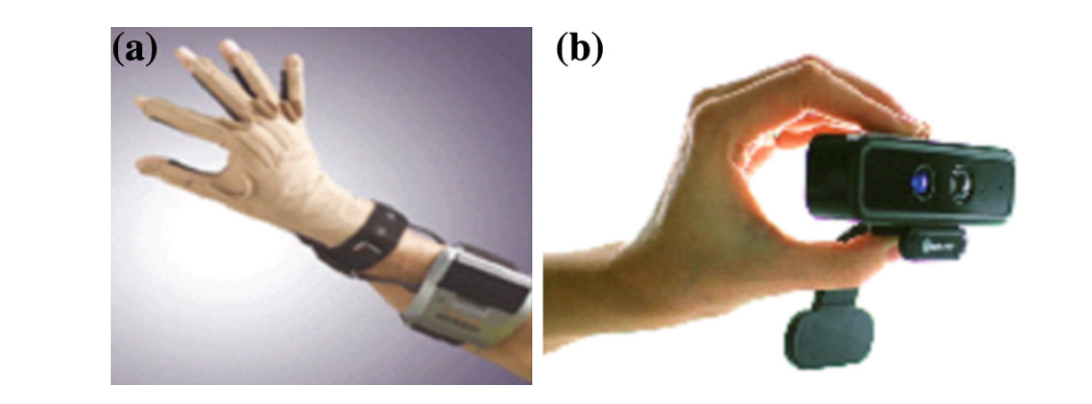
\includegraphics[width=0.6\linewidth]{fig1.png}
  \caption*{(a)基于触觉的手势识别:Cyber Glove II\cite{kevin2004};(b)基于计算机视觉的手势识别: SoftKinetic HD 相机\cite{iisuSDK2012}。}
  \caption{不同的手势识别技术}
  \label{fig:gesture_techniques}
\end{figure}

我们观察到,RGB-D 手势识别的主要挑战可以归因于两个因素:(i)\textit{信息冗余 (IR)}。
在纠缠的时空空间中,冗余信息很难处理 \cite{zhou2023unified, LI2024110536}。利用耦合建模结构的模型通常会在训练期间学习背景、照明和表演者外观等不相关的特征 \cite{zhou2023unified},这可能会导致误导性分类 (图 ~\ref{fig:gap_sample})。尽管现有方法在训练数据集上表现良好,但在未见的场景中,它们的准确性会显著下降。这种差异凸显了一个关键的泛化问题,即模型在消除冗余信息方面遇到挑战,阻碍了与任务相关的细微手势特征提取。
(ii)\textit{信息缺失 (IA)}。模型难以区分具有高视觉相似性的手势 (图 ~\ref{fig:sim_sample})。虽然现有方法建议加入额外的线索,如姿势 \cite{wan2016chalearn,zuo2023natural} 和光流 \cite{narayana2018focus} 来增强手势识别,但这些方法的有效性仍然依赖于视觉,并且受到运动模糊和透视变化等问题的严重影响,特别是在区分视觉相似的手势时。
鉴于这些挑战,有必要开发一种有效的方法,最大限度地减少不相关的信息冗余,并解决整个手势识别过程中基本信息的缺失。

\begin{figure}[tb]
  \centering
  \subcaptionbox{同一手势类别具有不同的背景、照明和视角。\label{fig:gap_sample}}
  {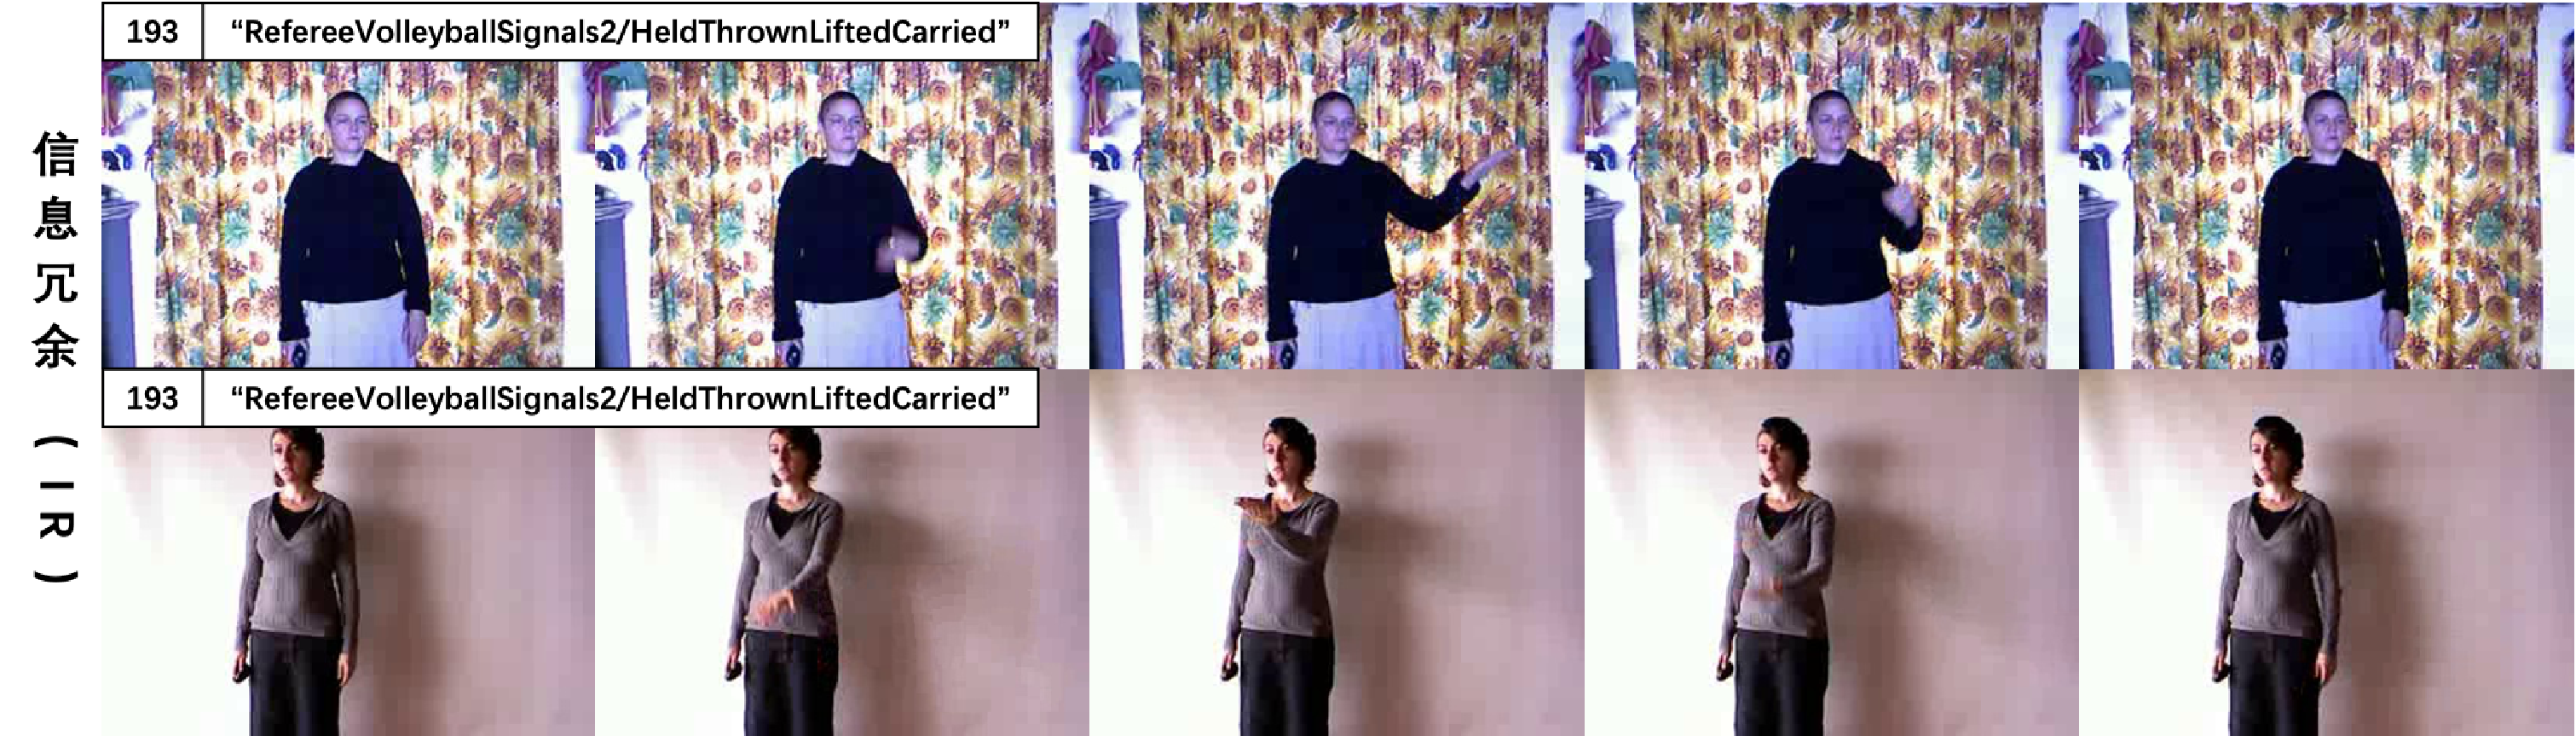
\includegraphics[width=1.0\linewidth]{IR.pdf}}
  \subcaptionbox{不同的手势类别具有视觉上相似的表示。\label{fig:sim_sample}}
  {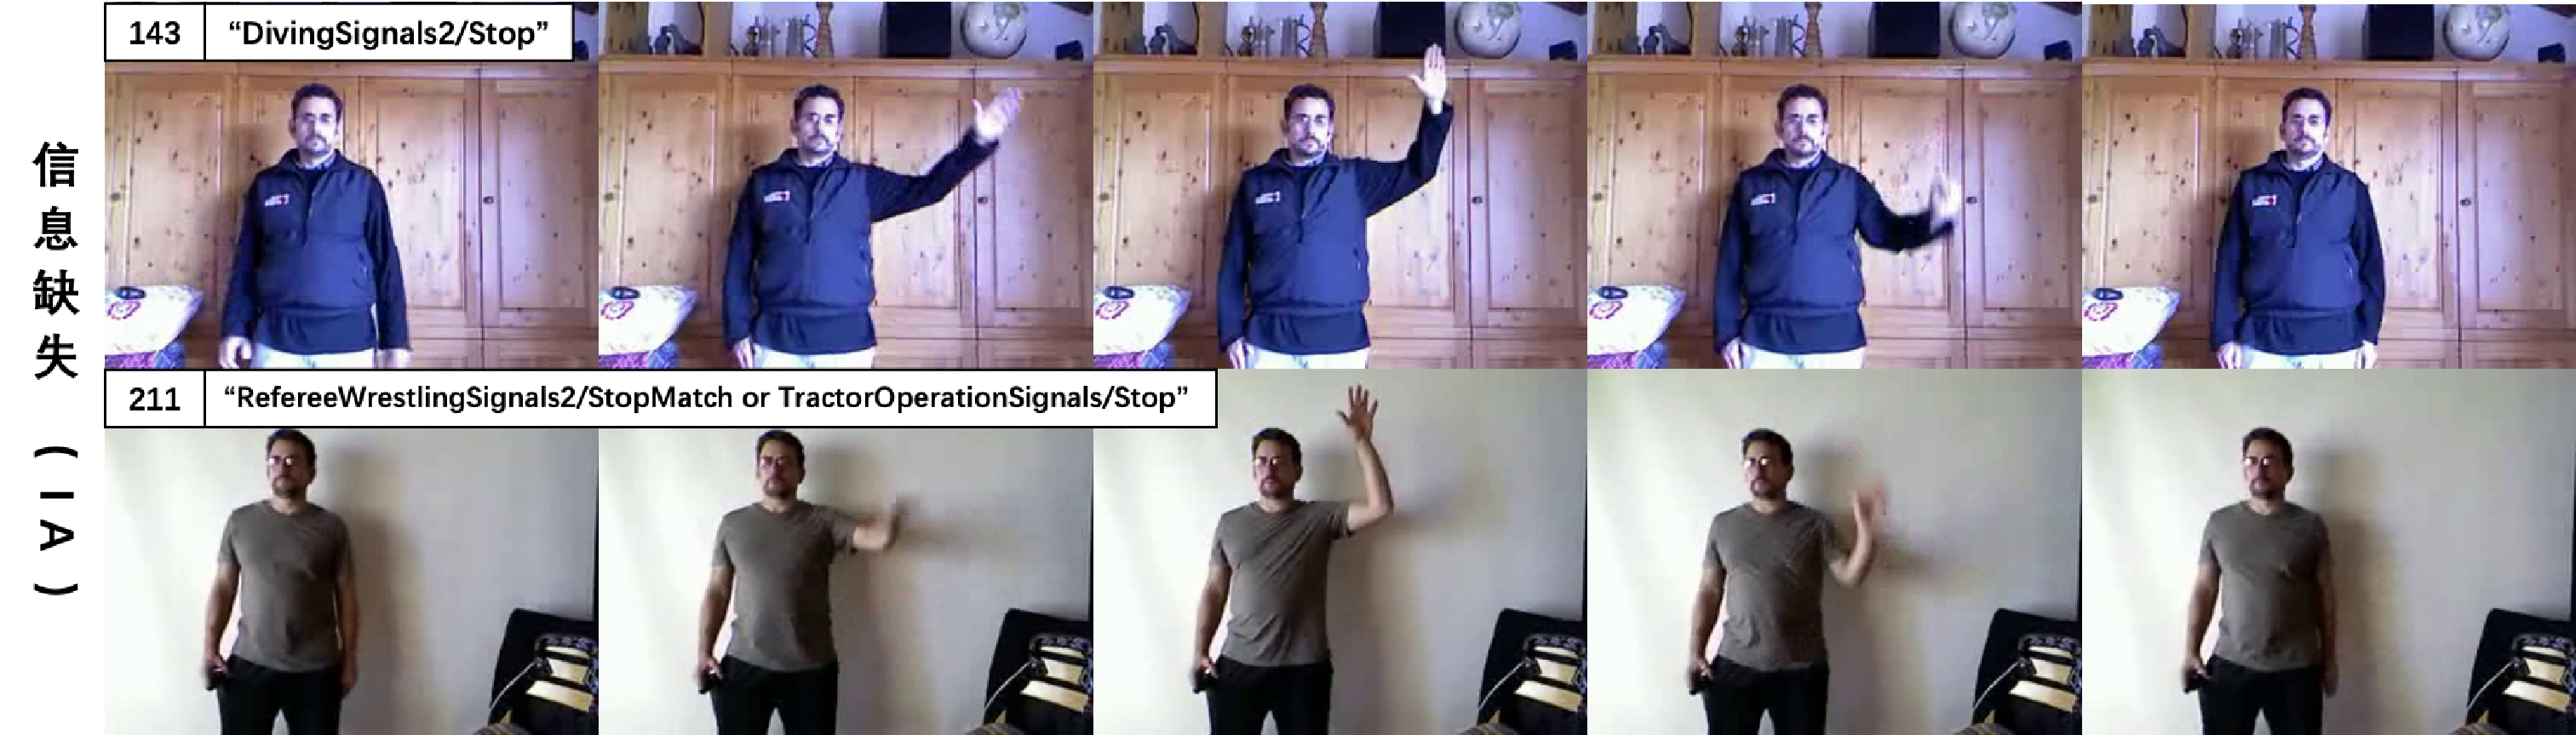
\includegraphics[width=1.0\linewidth]{IA.pdf}}
  \caption{RGB-D 手势识别的主要挑战可归因于两个因素:(i)\textbf{信息冗余 (IR)} 存在于类内,尤其是背景、照明和视角。(ii) \textbf{信息缺失 (IA)} 存在于类间,尤其是视觉上相似的手势。}
  \label{fig:samples}
  \end{figure}


\textbf{手势生成}因其在人机交互领域的广泛应用而备受关注,如虚拟现实、游戏和数字虚拟人等。为了增强手势生成的多样性和可控性,研究人员探索了多种模态,包括语音~\cite{yang2023diffusestylegesture, yang2023unifiedgesture,xu2025mambatalk}、文本转录~\cite{zhi2023livelyspeaker, pang2023bodyformer,liu2024emage}、情感~\cite{qi2024emotiongesture, qi2024weakly}、风格~\cite{ao2023gesturediffuclip, yang2023diffusestylegesture, ghorbani2023zeroeggs}以及说话者身份~\cite{yang2023diffusestylegesture+}等。其中,语音同步性和语义相关性是两个备受关注的关键方面。尽管深度神经网络~\cite{liu2024emage, xu2025mambatalk, cheng2024siggesture}的进步显著提高了生成质量和多样性,但当前的方法主要关注自发性的伴随语音手势,而忽视了文本驱动的非自发性手势~\cite{yang2024freetalker}。这通常导致虚拟人动作的模糊性~\cite{chen2024syntalker},并限制了通过文本提示控制生成动作的灵活性,阻碍了手势生成算法的实际应用。

一个关键挑战在于现有手势数据集缺乏直接的描述性文本标注:虽然语音数据自然且直接可用,但语义相关性通常仅通过语音转录推断,导致语义关联较弱。此外,手动标注手势语义成本过高,这阻碍了高质量生成和精细化的说话者语义控制。虽然一些方法尝试通过引入额外的动作数据集进行联合训练来缓解这一问题~\cite{yang2024freetalker},但它们仍然存在手势数据的语义差距,只能在两个任务之间切换而非实现联合控制。另一种潜在的解决方案是通过动作-文本对齐预训练构建对齐的嵌入空间,以获取手势的隐式文本标签~\cite{chen2024syntalker},但这会引入额外的训练和推理成本。此外,由于人体动作数据集和手势数据集之间存在显著的分布差异~\cite{chen2024syntalker},联合嵌入空间的泛化能力仍有待验证。鉴于这些挑战,有必要开发一种有效的方法,既能解决手势数据标注缺失问题,又能实现多模态信号的协同生成控制,同时将成本降至最低。


基于上述背景,本文致力于提出一种新颖的多模态手势识别与手势生成算法,并基于此开发一个交互式手语学习助手系统。首先,通过引入一种多策略解耦与语义集成手势识别网络,实现手势识别的准确性提升;其次,通过提出一种描述驱动的协同手势生成网络,增强手势生成的描述性控制;最后,通过在手语学习系统中集成手势识别和生成算法,实现手语动作的智能评估和标准动作库的动态扩充生成。该系统能够有效缓解手语教学资源匮乏的问题,提升自主手语学习的效率和质量,还可以为听障人士的日常交流提供有力的技术支持,具有重要的社会价值和广阔的应用前景。



\section{国内外研究现状综述}
\subsection{多模态动态手势识别}
\subsubsection{手势识别概述}
% 手势
手势是人类传递信息、表达意图的重要途径,文献\cite{kaaniche2009gesture, rautaray2015vision}将手势分类为两种类型:静态手势和动态手势。静态手势被定义为在任何时间内没有在空间中的方向和位置运动,如果上述时间持续时间有运动,则称为动态手势。动态手势又包括五种类型\cite{ottenheimer2018anthropology}:标志,情感展示,调节器,适配器和解释器。图\ref{fig:gesture_taxonomies}显示了手势类别的分类学。由于动态手势中往往包含更丰富的语义表示,近年来更多的研究围绕动态手势展开。
\begin{figure}
  \centering
  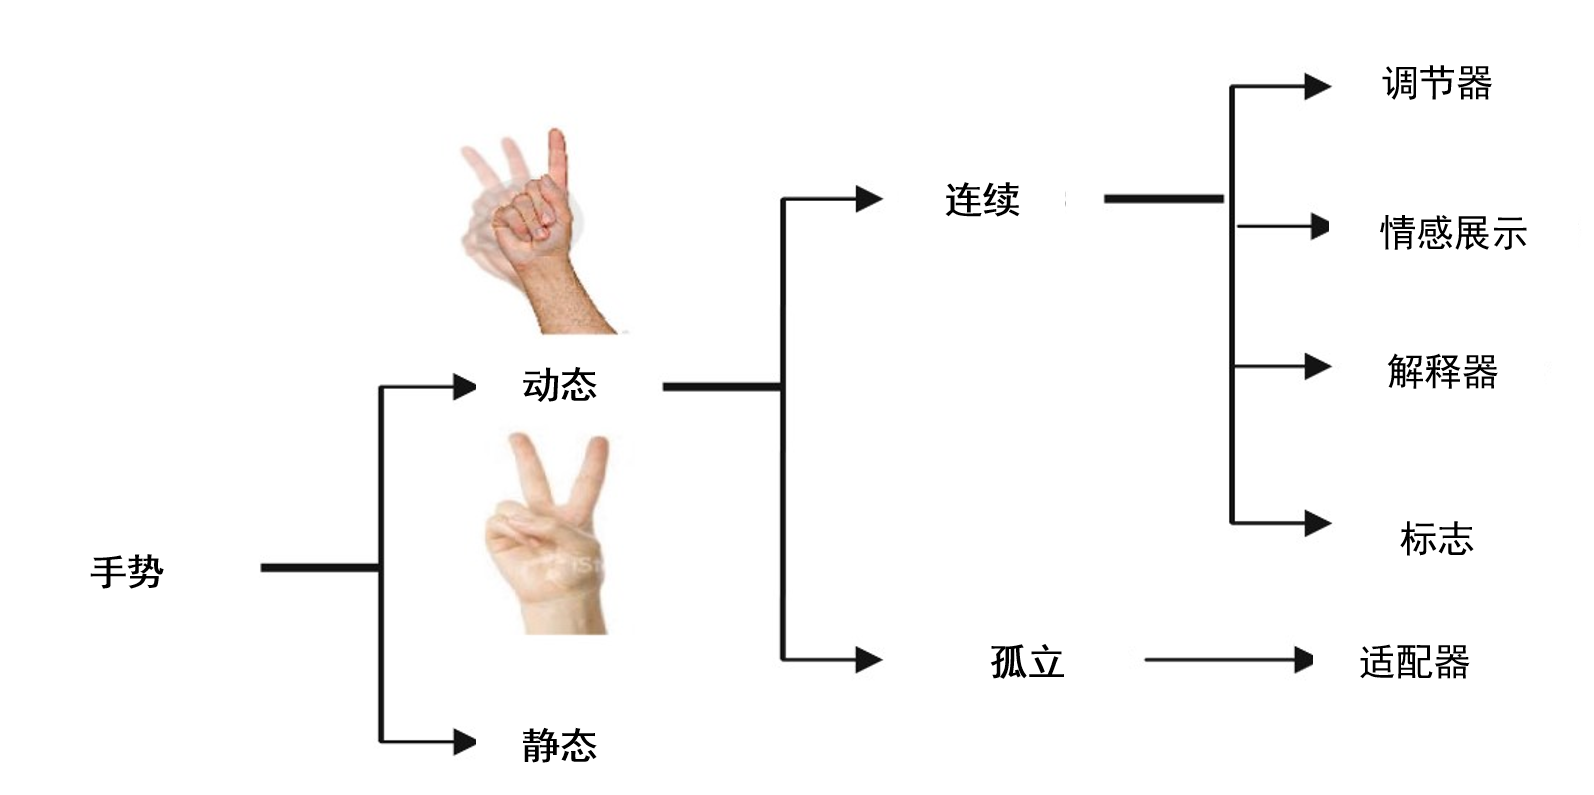
\includegraphics[width=0.9\linewidth]{fig2.png}
  % \caption*{}
  \caption{基于视觉的手势分类法\cite{rautaray2015vision}}
  \label{fig:gesture_taxonomies}
\end{figure}

% 手势识别
手势识别是一个完整的过程,涉及跟踪手势、识别其含义并将其转化为有意义的指令\cite{rautaray2015vision}。
%% 触觉、视觉
手势识别的主要方法可以分为基于触觉的方法和基于视觉的方法\cite{oudah2020hand,rautaray2015vision}。
基于触觉的方式是通过数据手套等设备检测手部动作、弯曲时的物理反应,收集相关数据并通过计算机或微控制器进行处理识别的方法。常用的接触式传感方法包括:数据手套、手部光学标记、加速度计、触摸屏、表面肌电等\cite{oudah2020hand}。
尽管基于数据手套的方法具有可穿戴、灵活便捷等优势,但它们也有许多局限。例如:基于接触的设备并没有给用户提供太多的可接受性\cite{rautaray2015vision},并且不适合老年人;电线连接会影响设备的灵活性;长时间使用也受到设备寿命的限制;此外,一些传感器可能相当昂贵\cite{oudah2020hand}。
视觉手势识别是通过相机等视觉传感器捕捉手势的形状和动作,并运用计算机视觉技术对2D和3D手势进行识别的过程。
常用的视觉相机设备包括2D摄像头、Kinect、LeapMotion、Time of Flight (ToF) 相机等\cite{基于视觉的动态手势识别研究综述}。
尽管视觉手势识别容易受到遮挡、光照等问题的干扰,但由于其具有用户友好、设备易得的优势,因此视觉手势识别成为近年来研究的主流方向。

本研究将深入探讨基于视觉的动态手势识别,探讨多模态识别过程中的特征解耦与融合,通过引入先进的深度学习技术进一步提升识别的准确性和鲁棒性。
%此外,由于手势动作往往涉及相当多的自由度(DoF),即使是相同的手势在不同视点下也会发生2D外观的巨大变化,不同的手势动作可能存在不同的空间分辨率与手势速度\cite{rautaray2015vision},不同的背景与手势表演者也会给识别增添困难...... ,因而视觉手势识别研究对于科研人员来说仍然具备相当多的挑战性\cite{基于视觉的动态手势识别研究综述}。
%% 动态、静态
%% 连续、孤立
% 输入模态
% ...
% 文献评述

\subsubsection{基于手工提取特征的手势识别方法}
% ref: rautaray2015vision
% ref: 基于视觉的动态手势识别研究综述
早期研究使用手工提取特征进行手势识别,包括检测、追踪和识别三个阶段\cite{rautaray2015vision}。
检测的目的是进行手的检测和相应图像区域的分割,常基于肤色\cite{sigal2004skin}、形状\cite{chen2007real}、3D模型\cite{tekin2019h+}、运动\cite{pun2011real}、骨架\cite{jiang2021chal21}等特征进行手部检测。
追踪技术旨在获取手部在连续帧中的位置信息,构建动态轨迹特征。通过对这些包含手势基本信息的轨迹进行分析,可实现对手势类型的识别与理解。
基于模板的方法(Template based)\cite{crowley1995finger}与手部检测方法非常相似。此类方法在前一帧中检测到手的空间附近调用手检测器,从而在很大程度上限制图像搜索空间,但要求图像具有足够的采样帧率。基于最佳估计的方法(Optimal estimation)\cite{argyros2004real}采用卡尔曼滤波器\cite{kalman1960new}提供的最优估计框架具有实时的性能并能为连续帧提供预测。基于粒子过滤(Particle filtering)的方法\cite{perez2002color}被用来在密集的视觉混乱中跟踪手的位置和手指的配置,此类方法用一组粒子建模手的位置,对于复杂的模型需要更多的粒子。基于连续自适应均值偏移(CamShift)的方法\cite{wang2010study}参考了基于核的mean shift算法原理,通过迭代搜索找到帧序列中与其样本模式最相似的分布模式来跟踪目标,并能够在跟踪过程中自适应调整跟踪窗口的大小和目标的分布模式。CamShift具有轻量、鲁棒、高效的优点,但在复杂场景中容易失败、且容易发生窗口漂移问题。
识别阶段的目标是对手的位置、姿势提供最终的语义解释。静态手势识别可以使用模板匹配或基于机器学习的简单分类器\cite{基于视觉的动态手势识别研究综述},如:支持向量机(SVM)\cite{burges1998tutorial}、随机森林\cite{基于视觉的动态手势识别研究综述}、K近邻算法(KNN)\cite{thirumuruganathan2010knn}等。动态手势识别则需要对时间维度进行建模,隐马尔科夫模型(HMM)\cite{liang1996sign},动态时间规整(DTW)\cite{corradini2001dynamic},时延神经网络\cite{sigal2004skin}等算法在动态手势识别系统中得到了广泛的应用。
传统手势识别方法的关键在于如何合理地提取手工特征,具有计算成本低、速度快的优势。但由于过于依赖于技术人员经验与精巧的模型设计,算法的泛化性、鲁棒性往往较差。

\subsubsection{基于深度学习的手势识别方法} % (时空建模)
伴随着计算能力的提升以及大规模多模态数据的积累,基于深度学习的手势识别技术实现了重大突破。
与传统算法相比,深度学习不仅减少了对手工工程的需求,而且提升了算法的准确性、适用性与效率。因此,基于深度学习的手势识别方法已经成为该领域的主流研究方向,受到广泛关注。

% \paragraph{基于RGB-D的动态手势识别}
% ref: 基于视觉的实时手势识别方法(2019大连理工)
% RGB
%% 2DCNN
卷积神经网络(CNN)已被证明是许多计算机视觉任务中的有效算法,2DCNN方法被广泛用于处理静态手势图像的分类和识别任务。这些网络通过卷积层和池化层有效地捕获图像中的空间特征。
%% Two stream
针对视频中的动态手势动作,早期研究者试图在时域中扩展 2DCNN 的连接性以进行视频分类\cite{karpathy2014large}。Simonyan等人\cite{simonyan2014twostream}提出了双流神经网络(Two Stream CNN)来分别学习空间和时间特征,其中空间流处理静态单帧图像,时间流则处理多帧光流。
TSN\cite{wang2016tsn}在双流卷积神经网络的基础上进行稀疏时间采样,所提出的时间段网络可以对整个动作视频进行高效的学习。
TRN\cite{zhou2018trn}进一步改进了TSN中的融合方式,并提出了时间维度上的多尺度特征融合,以提升算法的鲁棒性。
2DCNN结构简单,但存在时域信息建模的不足;而双流方法依赖于预先提取的密集光流进行运动表示,网络同样缺乏有效的时域特征提取模块。

%% 3DCNN
受图像识别领域卷积神经网络突破的启发,3DCNN被提出并广泛应用于视频理解任务。
C3D网络\cite{tran2015c3d}通过在时空维度上扩展二维卷积核,实现了对视频序列中时空特征的直接提取,该网络在多种视频分析任务中展现出优异的性能。
此后,一系列基于3DCNN的神经网络被提出,并逐渐成为视频理解任务中的主流选择。
Carreira等人\cite{carreira2017i3d}结合了双流神经网络与3DCNN的优势,引入了一种新的双流膨胀 3D ConvNet (I3D)进行时空建模,在Kinetics动作视频数据集上实现了最先进的水平。
R2+1D\cite{tran2018r2+1d}通过将3D卷积分解为2D空间卷积和1D时间卷积的方式,实现了更高效的时空特征提取。
S3D\cite{xie2018s3d}考虑速度与准确度之间的平衡,将I3D与时空分离卷积结合,并引入一种特征门控机制以进一步提升网络的识别准确率。
Zhang等人提出了Deformable 3DCNN\cite{zhang2020deformable3d},通过所设计的轻量级时空可变形卷积模块,通过根据前序特征图学习额外的偏移量来增强3D卷积的时空采样位置,以减轻手势识别中背景的干扰。
3DCNN能够有效提取视频中的局部时空特征,但对长序列数据的建模能力较弱。此外,当网络输入较长时,往往需要更多层或更大的内核和步幅大小,增加了网络计算成本的同时也容易出现过拟合现象。

%% Recurrent
循环神经网络(RNN)\cite{jozefowicz2015empirical}和长短期记忆网络(LSTM)\cite{yue2015beyond}是处理序列数据的常用模型。
这一特点促使研究人员将 CNN 和 RNN/LSTM 的优势结合起来,先后学习局部和全局时空特征。
长期循环卷积网络(LRCN)\cite{donahue2015lrcn}依次使用卷积神经网络(CNN)和长短期记忆(LSTM)网络学习空间和时间特征,多提出的方法在动作识别、图像描述与视频描述多任务中取得了有竞争力的结果。
Molchanov\cite{molchanov2016online}和Cao\cite{cao2017egocentric}等人分别将3DCNN与循环神经网络(RNN)和长短期记忆网络(LSTM)相结合以进行端到端的手势识别,前者可以从多模态数据中同时检测和分类动态手势,后者则额外设计了一个具有相邻时间片之间循环连接的时空转换模块,可以在空间和时间维度上主动地将三维特征图转换为规范视图。

%%% ConvLSTM
由于全连接长短期记忆网络(FC-LSTM)难以提取数据中的空间特征,Shi等人\cite{shi2015convlstm}提出了卷积长短期记忆网络 (ConvLSTM) 来处理连续图像以进行临近降水预报。
研究表明,相比LSTM,ConvLSTM能更有效地捕获时空特征,并已在动作识别、手势识别等多个视觉任务中得到成功应用。
Zhu等人\cite{zhu2017multimodal}提出了一种基于3D卷积和ConvLSTM的孤立手势识别方法。该方法首先利用3DCNN提取短期时空特征,随后通过ConvLSTM建模长期时空依赖关系,并采用SPP\cite{he2015spatial}对特征进行归一化。该方法分别在RGB和深度模态上训练,最终通过平均融合得到预测结果。
在此基础上,Zhang等人\cite{zhang2017learning}提出了3DCNN+BiConvLSTM+2DCNN网络用于孤立手势识别。具体地,文章引入了双向卷积长短期记忆网络(BiConvLSTM)以替换网络中的ConvLSTM,并引入额外的2DCNN学习更高层次的时空特征。
AttnConvLSTM\cite{zhang2018attention}与
ConvLSTMForGR\cite{zhu2019redundancy}进一步探索了ConvLSTM中空间卷积的冗余性以及注意力机制的影响。
研究发现,门控结构中的空间卷积对特征融合的作用有限,同时在输入输出门中引入注意力机制也未能有效提升特征融合效果。
在此基础上衍生出一种新的GatedConvLSTM变体,其中卷积结构仅嵌入到ConvLSTM的输入到状态转换中。
对于未经分割的手势视频,Zhu等人\cite{zhu2018continuous}进一步将类似网络应用于连续手势识别,并提出了一种两阶段的连续手势识别方法。在分割阶段,使用时间扩张三维卷积神经网络将连续手势序列分割成孤立的手势实例;在识别阶段,则使用基于3DCNN+ConvLSTM+2DCNN的孤立手势识别网络进行识别分类。
基于循环神经网络的动态手势识别方法能够有效进行长期时间建模。然而由于手势视频中不同阶段的帧往往具有不同的重要性\cite{lin2018large},此类方法因为缺少时域上的注意机制,难以对不同重要性的视频帧进行有效建模。
另外,这类网络的计算效率也受到限制,因为每个时间步的计算都需要等待前一步的结果。

Transformer架构\cite{vaswani2017attention}可以通过注意机制更好地捕获上下文信息。
Vision Transformer(ViT) \cite{vit2021image}是一项开创性的工作,通过将视觉数据作为序列处理,而不是依赖于传统的卷积网络,引入了图像分类的新范式转变。
受ViT的启发,Video Transformer(VT)\cite{selva2023video} 通过引入额外的时间维度进行时空建模与视频理解。
TimeSformer\cite{bertasius2021space}率先使用纯Transformer结构用于视频识别。ViViT\cite{arnab2021vivit}探索了几种不同的时空注意力分解变体,验证了时空编码器分离方法的有效性。VTN\cite{neimark2021video}同样采用时空编码器分离的方式,并进一步引入Longformer实现复杂度为O(n)的长序列建模。
该机制通过滑动窗口实现局部上下文的自注意力计算,并结合任务相关的全局注意力机制。
Video Transformer(VT)方法已经在行为识别等视频理解领域取得了显著的成功,然而目前却少有研究将Video Transformer方法应用于手势识别领域来解决动态手势的分类问题。这可能是由于Video Transformer在计算复杂性方面面临着挑战,通常需要大量的计算资源和大规模的数据集来实现最佳性能\cite{khan2022transformers}。

% 受上述工作的启发,本研究将循环神经网络(ConvLSTM)与视频变换器(VT)的优势结合起来,引入了一种基于循环的手势识别变换器(RGRT,Recurrent Gesture Recognition Transformer),以实现多尺度的时空注意力建模。我们利用时域窗口变换器(TWT,Temporal Window Transformer)在局部片段内进行并行计算,在全局视频范围内则使用基于卷积长短期记忆网络的循环结构进行长期建模,从而在保证计算效率的同时提升网络的识别性能。
与以前利用耦合建模结构来处理纠结的跨模态特征的方法相比,本研究侧重于两个解耦维度中的多模态特征的相互作用,并且可以无缝集成到各种 RGB-D 方法中。


% \subsubsection{\textcolor{red}{基于三维骨骼数据的手势识别}}
% %多模态:skeleton,点云,...
% 随着更多的多模态手势数据集被提出,除了主流的基于RGB-D视频的手势识别方法外,近年来也涌现出了许多基于3D骨架、点云等模态数据的方法。
% Aich等人提出了一种基于无数据类增量学习的三维骨骼序列手势识别方法(DFCIL)\cite{aich2023data},并引入了一种简单有效的用于DFCIL模型反演的边界感知原型采样机制。
% Liu等人\cite{liu2023temporal}则提出了一种时间解耦图卷积网络(TD-GCN)进行三维骨骼序列手势识别,它对来自不同帧的骨架应用不同的邻接矩阵。
% Min等人\cite{min2020efficient}将手势识别作为一个不规则序列识别问题,旨在捕获点云序列之间的长期空间相关性。所提出的PointLSTM在多个骨架数据集上取得了具有竞争力的结果。
% %% 解耦 Decoupled
% Bigalke等人\cite{bigalke2021fusing}认为直接处理三维点云序列有利于手势识别,并提出了一种解耦的双流模型分别进行局部姿势特征与全局运动特征的学习,多尺度的特征最终被融合在LSTM中用于时间建模。
% 类似地,Liu等人\cite{liu2020decoupled}提出了一个解耦的端到端双流网络进行基于骨骼的手势识别。网络将手势解耦为手部姿势变化和手部运动,然后分别建模。对于前者,骨架序列被嵌入到3D手部姿势演化体(HPEV)中使用3DCNN提取细粒度的姿势变化特征;对于后者,手中心和指尖的移动被安排为一个2D手部运动图(HMM),使用2DCNN捕捉整体运动;并最终将两个流的预测结果聚合。

% % 文献评述
% % \subsubsection{基于解耦的动态手势识别}
% 文献\cite{bigalke2021fusing, liu2020decoupled}已经明确指出,对于动态手势的解耦对提升手势识别性能具有积极作用。目前,解耦手势识别的研究主要集中在三维骨架手势方面,然而,三维骨骼数据的获取成本较高,需要依赖于上游的三维人体姿态识别算法或大量人工标注,限制了其在实际应用中的推广。相比之下,目前尚未有专注于二维手势视频的解耦手势识别研究。

\subsubsection{解耦手势特征学习}
由于复合手势特征在纠缠空间\cite{zhou2023unified,LI2024110536}中难以处理,一些研究人员尝试从各个角度解耦复杂手势特征学习,以提高识别性能。
一些工作\cite{zhou2022decoupling,LI2024110536} 尝试将“时空”手势特征空间解耦。
Zhou 等人 \cite{zhou2023unified} 提出了一种解耦时空表示学习网络 (DSN, DTN) 来学习特定于维度的表示。
然而,明确地隔离整个网络的时空维度可能会破坏特征的时空连通性,从而损害模型捕获隐式关节时空信息的能力。
% pose-motion
其他一些研究侧重于将 3D 手势表示与 3D 骨架或点云数据解耦。
Guo 等人 \cite{GUO2021108044} 强调,可以从两个角度看到手部骨架:显式关节云和隐式骨架拓扑。
Liu 等人\cite{liu2020decoupled} 提出,各种手势类别在对不同尺度特征的依赖方面表现出多样性。
Bigalke 等人 \cite{bigalke2021fusing} 提出了一种解耦的双流模型,用于从 3D 点云序列中独立学习局部姿势特征和全局运动特征。
然而,这种方法受到高数据收集成本的限制,对实际应用提出了挑战。
本研究试图同时将 RGB-D 手势与两个范例分离:i) 姿势-运动解耦 (PMD) 和 ii) 空间-时间-通道解耦 (STCD)。
这种方法有效地将细微特征集成到两个子空间中,同时保留了联合特征,使其有别于其他方法。

\subsubsection{多模态视觉-语言模型}
随着多模态领域的蓬勃发展,大量视觉语言模型 \cite{radford2021learning, li2022blip} 应运而生,并被应用于各种任务,例如,图像文本匹配和图像文本检索。
CLIP \cite{radford2021learning} 是该领域的开创性工作之一,利用大规模图像文本对进行训练,共同优化文本编码器和视觉编码器,以实现图像和语义特征对齐。
鉴于 CLIP 依赖于大规模预训练,一些研究人员旨在基于 CLIP 进行微调,以实现高效的少样本迁移和领域泛化 \cite{gao2024clip}。
Zuo 等人 \cite{zuo2023natural} 避免使用密集文本编码器,而是选择使用 fastText 来提取词级嵌入,以利用注释(符号标签)中包含的隐性知识。
手势本身具有自然的语义属性;然而,使用简单的词级嵌入不足以捕捉手势注释的复杂性。
在这一努力中,我们首先将语义引入手势识别,利用预先训练的 CLIP 和适配器从手势注释线索中提取更丰富的语义,并促进语义视觉特征的充分交互,这与以前的视觉语言模型不同。


% 本文旨在填补基于二维手势视频的解耦手势识别研究领域的空白。通过采用手势分割方法并引入一种基于手部骨架弯折编码的手势表示(SBCGR),我们将动态手势视频解耦为细粒度的局部姿势变化和粗粒度的手部运动。对于这些不同尺度的特征,我们采用多流网络进行特征提取与识别。这一研究框架不仅能够为视觉动态手势识别领域提供关于基于二维数据的手势解耦方法的新见解,还能够丰富动态手势识别算法的应用场景。



\subsection{协同手势运动生成}

\subsubsection{手势生成概述}
手势生成任务是从多模态数据中生成手势动作序列的复杂任务。为了实现更多样、可控的协同语音手势生成,多模态数据被辅助建模,包括语音音频~\cite{yang2023diffusestylegesture, yang2023unifiedgesture,xu2025mambatalk}、文本转录~\cite{zhi2023livelyspeaker, pang2023bodyformer,liu2024emage}、情感~\cite{qi2024emotiongesture, qi2024weakly}、风格~\cite{ao2023gesturediffuclip, yang2023diffusestylegesture, ghorbani2023zeroeggs}、说话人ID~\cite{yang2023diffusestylegesture+}。其中,语音同步性和语义相关性是两个关键方面。由于语音数据的自然可获得性,协同语音手势生成一直是主要的研究重点。然而,由于手势数据集缺乏直接的描述性文本标注,语义相关性通常只能通过语音转录来推断,这限制了语义关联的强度。
Yang等人\cite{yang2024freetalker}提出了一种协同语音和文本驱动的方法,但仍然受到标注不足的限制,且无法提供基于两种信号的协同生成。Chen等人\cite{chen2024syntalker}利用提示-动作对齐预训练来生成隐式文本标签,但引入了额外的训练和推理成本。与现有方法不同,我们提出了一种基于描述的手势潜在扩散模型,在保持低标注和计算成本的同时,实现了语义相关性和节奏一致性。

为了解决这些限制,我们提出了一种联合描述和语音驱动的协同手势生成框架,在实现生成手势的语义相关性和节奏一致性的同时,保持低标注和计算成本。

\subsubsection{基于深度学习的手势生成方法}
传统方法依赖基于规则或统计模型来学习语音-手势映射,而深度学习方法利用神经网络来建模音频和手势之间的复杂关系\cite{nyatsanga2023comprehensive}。

早期方法主要采用RNN\cite{liu2022beat,yoon2020speech}进行手势序列建模。
Liu等人\cite{liu2022beat}提出了一个大规模身体-表情-音频-文本数据集 BEAT,它具有 76 小时的高质量多模态数据。基于此他们构建了一个级联运动网络 (CaMN),它由上述六种模态组成,这些模态以级联架构构建,用于手势合成。
Yoon等人\cite{yoon2020speech}引入了一种基于多模态上下文的手势生成方法,通过融合语音、文本和说话者特征来生成自然的手势动作。
但基于RNN的方法在捕获长期依赖性和计算效率方面存在诸多局限
。随后,Transformer\cite{zhi2023livelyspeaker, pang2023bodyformer}被引入以通过自注意力机制更好地建模时序关系。
Zhi等人\cite{zhi2023livelyspeaker}引入了 LivelySpeaker,这是一个实现语义感知协同语音手势生成的框架,并提供了多个控制句柄。该方法任务分为两个阶段:基于脚本的手势生成和音频引导的节奏优化。
Bodyformer\cite{pang2023bodyformer}提出了一个变分转换器来有效地模拟手势的概率分布,这可以在推理过程中产生不同的手势,并引入了一个模式位置嵌入层和一个模态内预训练方案来捕捉不同说话模式下的不同运动速度并缓解数据的稀缺性,以从有限的数据中学习语音和 3D 手势之间的复杂映射。
然而,Transformer首先于其相对于序列长度的二次方复杂度,带来了显著的计算挑战。
近期,MambaTalk\cite{xu2025mambatalk}首次将选择性状态空间模型(SSM)引入手势合成领域,通过线性时间计算实现了高效的序列建模。该方法实现了具有离散运动先验的两阶段建模策略,以提高手势的质量。利用基础 Mamba 块,通过多模态集成增强手势多样性和节奏。

为了提升生成质量和可控性,研究者开始探索基于潜变量的生成方法。一些方法采用VQ-VAE架构对手势动作进行离散编码,实现更高质量的手势生成。
EMAGE~\cite{liu2024emage} 利用四个合成VQ-VAE与掩码身体手势先验来提高结果的保真度和多样性,该研究同时引入了BEAT2(BEAT-SMPLX-FLAME),这是一个新的网格级整体共语音数据集,优化了头部、颈部和手指运动的建模,提供了社区标准化的高质量 3D 动作捕捉数据。
QPGesture~\cite{yang2023qpgesture}提出了一个手势 VQ-VAE 模块来学习codebook来总结有意义的手势单元。每个代码代表一个独特的手势,有效缓解了随机抖动问题。
TalkSHOW~\cite{yi2023generating}提出了一个新颖的语音到动作生成框架,其中分别对面部、身体和手进行建模,结合VQ-VAE和跨条件自回归模型(Gated PixelCNN)产生连贯且一致逼真的运动。

由于其强大的生成能力,扩散模型\cite{cheng2024siggesture,alexanderson2023listen,tevet2022mdm,yang2023diffusestylegesture}近期被广泛应用于运动和手势生成,显著增强了生成输出的多样性。
SIGGesture~\cite{cheng2024siggesture}通过大规模预训练扩散模型的语义注入进行泛化协同语音手势合成。该研究收集了一个名为LSMoG的大规模手势数据集进行预训练,时间长达400小时。
在运动生成领域,MotionDiffuse~\cite{zhang2024motiondiffuse}代表了第一个基于文本的运动扩散模型,该模型提供了对身体部位的细粒度指令,并实现了随时间变化的文本提示的任意长度的运动合成。
MDM~\cite{tevet2022mdm}引入了一种基于原始运动数据的运动扩散模型,实现了高质量的生成和通用的条件化,共同构成了新的运动生成任务的良好基线。
Yang等人~\cite{yang2023diffusestylegesture}使用使用扩散模型生成风格化音频驱动的协同语音手势,可以生成自然、语音匹配、风格一致的手势。
然而,现有基于扩散的方法通常直接在动作空间进行建模采样,导致计算开销大且训练不稳定。相比之下,潜在扩散模型(LDMs)\cite{rombach2022high}通过在低维潜空间进行操作,在保持强大生成能力的同时实现了计算效率。

与现有方法不同,我们提出了一种基于描述增强的手势潜在扩散模型,该模型在保持低标注和计算成本的同时,实现了语义相关性和节奏一致性的双重目标。

\subsubsection{动作-文本转换}
人类动作展现出类似于自然语言的语义耦合,常被视为一种肢体语言形式~\cite{jiang2024motiongpt}。以往关于人体运动的研究探索了各种与文本相关的任务,包括文本到动作生成~\cite{tevet2022mdm,guo2022humanml3d}、动作到文本描述~\cite{jiang2024motiongpt,guo2022tm2t}以及统一的动作-语言建模~\cite{tevet2022motionclip,jiang2024motiongpt,jiang2024motionchain}。
近期的文本到动作工作(MDM~\cite{tevet2022mdm}、MLD~\cite{chen2023executing}、MotionLCM~\cite{dai2024motionlcm})利用预训练语言模型提取语义信息来控制动作生成。动作描述旨在使用自然语言描述人类动作,早期方法依赖统计模型和RNN来学习动作到语言的映射~\cite{takano2015statistical, yamada2018paired}。
近年来,双向动作-文本转换受到了更多关注。TM2T~\cite{guo2022tm2t}通过标记化首次实现了动作与文本的双向生成,尽管仅限于单一统一框架。随着大语言模型的发展,统一的动作-语言模型(如MotionGPT~\cite{jiang2024motiongpt}、MotionChain~\cite{jiang2024motionchain}、M3GPT~\cite{luo2024m})通过融合语言数据和大规模动作模型而涌现。

尽管手势本身具有自然的语义属性,但目前尚未有研究探索手势理解和描述生成。
为了解决这些局限性,本文首先探索了一种手势描述生成方法来填补手势数据中文本标注的空白,并开发了一种多粒度描述控制机制,实现对非自发手势的精确语义控制。



\subsection{基于手势的人机交互应用系统}
% Hand Gesture Recognition Based on Computer Vision: A Review of Techniques
% ref: 基于视觉的动态手势识别研究综述 解迎刚 1,2,王全 1
% ref: 伍杰2019基于视觉的实时手势识别方法研究
% ref: 审稿/人机交互.pdf
手势作为人与人之间交流的自然媒介形式,是人机交互最适合的形式之一\cite{oudah2020hand},基于手势的人机交互技术已经被广泛应用在各个领域。例如:

(1)机器人控制。 基于手势的人机交互,可被广泛用于机器人导航控制等领域\cite{al20223d}。国内无人机制造商大疆公司所发布的晓Spark的无人机可以识别用户手势,完成上下起降、左右移动和拍照等基本操作,极大的提高了用户体验(图~\ref{fig:3a})。

\begin{figure}
  \centering
  \subcaptionbox{大疆无人机晓 通过手势控制拍照\label{fig:3a}}
    {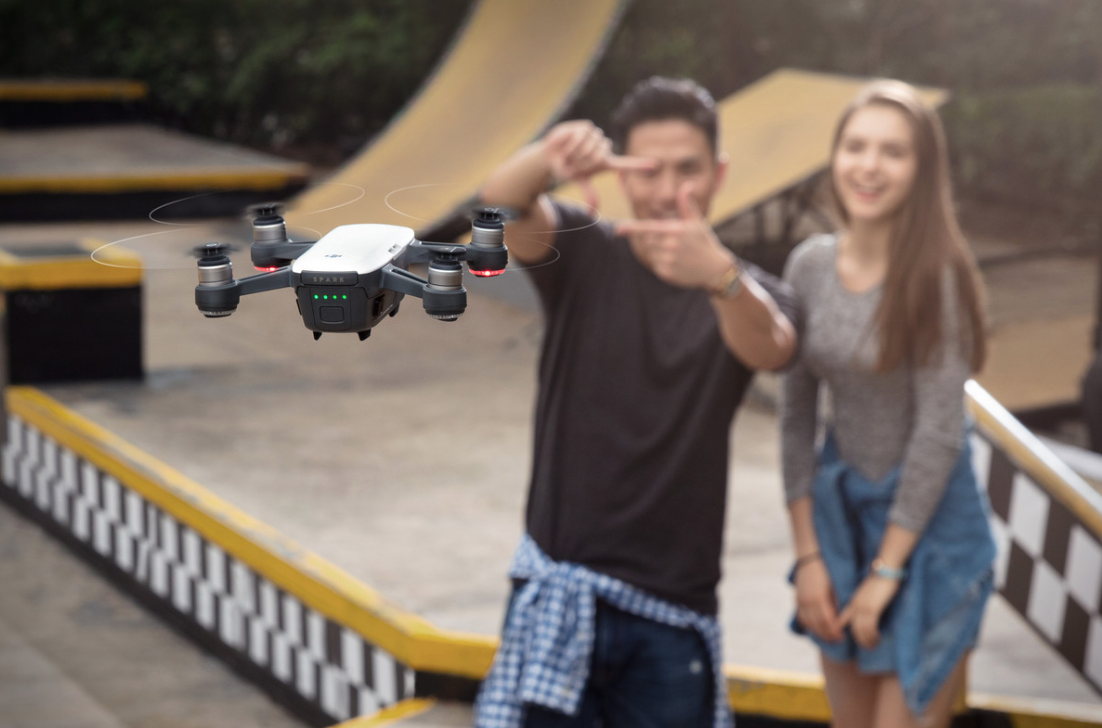
\includegraphics[width=0.4\linewidth]{fig3a.png}}
  \subcaptionbox{Oculus Quest手势追踪\label{fig:3b}}
    {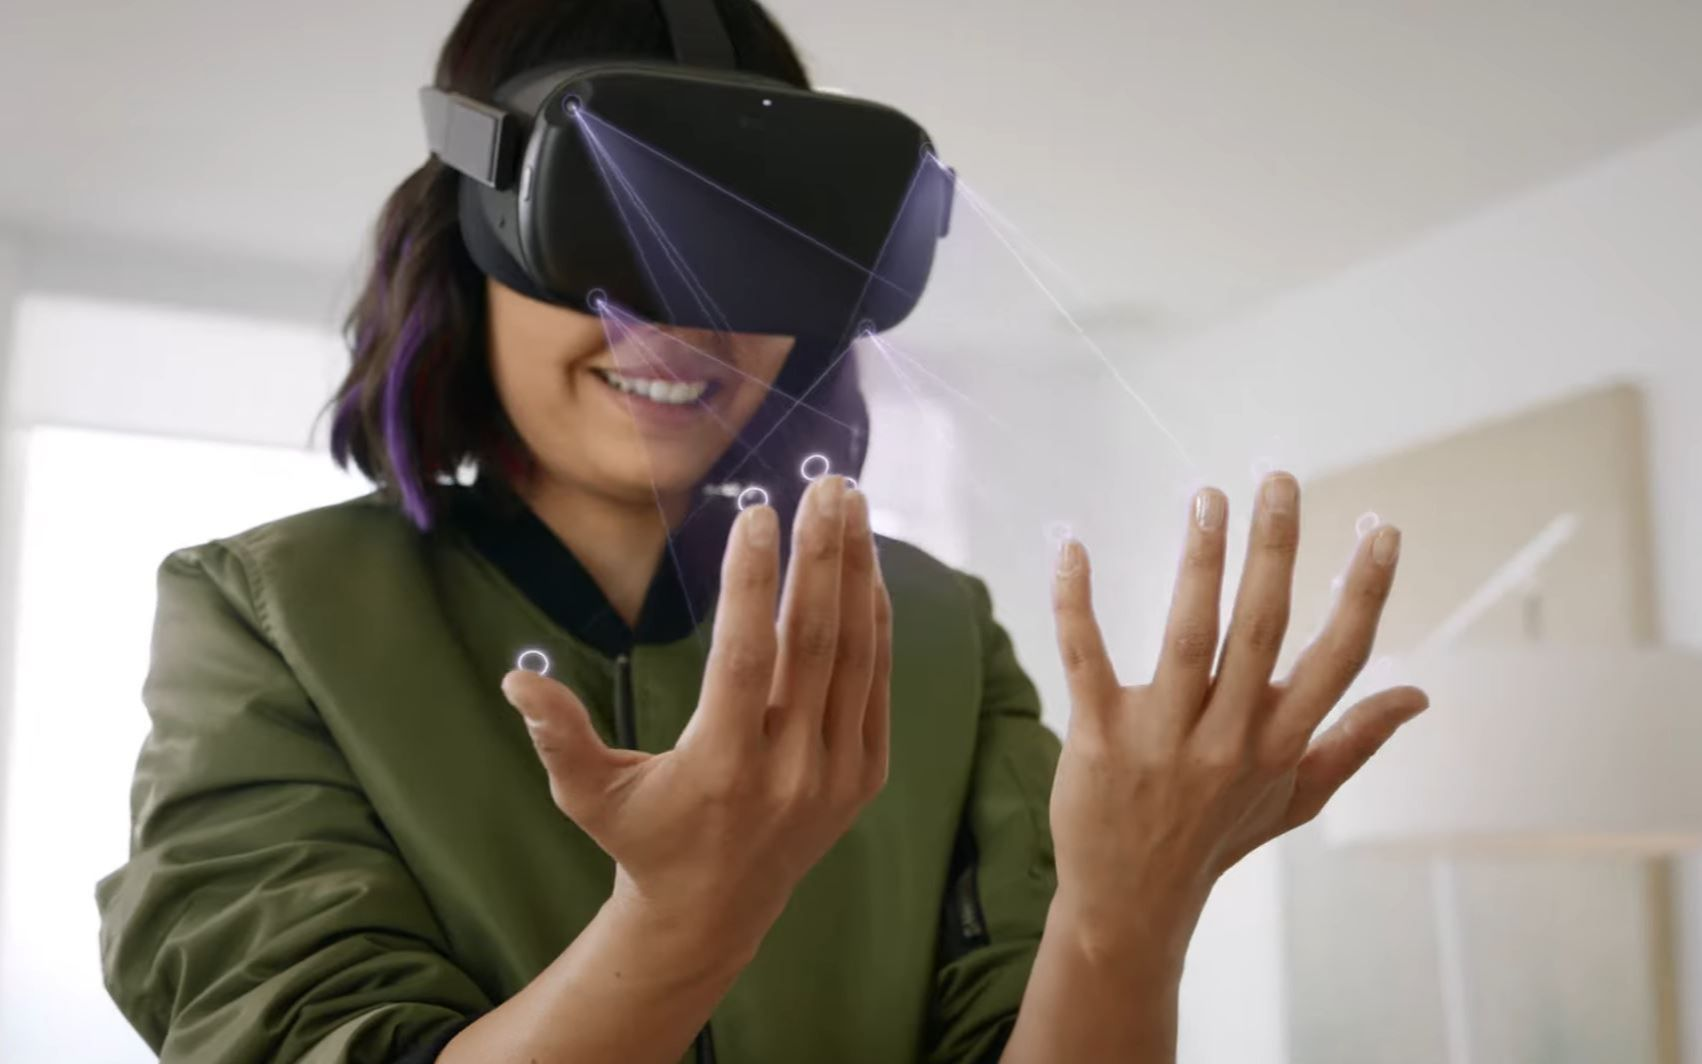
\includegraphics[width=0.4\linewidth]{fig3b.jpg}}
  \caption{基于手势识别的人机交互应用系统}
  \label{fig:HCI_system}
\end{figure}

(2)车载手势。Alba-Castro等基于手势识别技术, 构建了一个基于手势操作的车载娱乐媒体设备控制系统\cite{parada2014hand}。 Manawadu 等基于人车接口,利用手势识别的技术实现了自动驾驶汽车的经纬度控制\cite{manawadu2016hand}。
%[32] ALBA-CASTRO J L, GONZáLEZ-AGULLA E, PARADA-LOIRA F. Hand gestures to control infotainment equipment in cars[C]// Intelligent Vehicles Symposium. 2014. [33] MANAWADU U, KAMEZAKI M, ISHIKAWA M, et al. A hand gesture based driver-vehicle interface to control lateral and longitudinal motions of an autonomous vehicle[C]// IEEE International Conference on Systems. 2017.
% 宝马集团在 2015 年推出的车辆 iDrive 人机交互 指令系统,能够使用手势对车辆输入指令,如旋转手势进行音量调整、空中滑 动手指进行电话的接听等,实现对车辆的智能化控制。
% 君马 SEEK 5,9 种动态手势动作
% “Ez more 智能手势控制精灵” 

(3)智能家居。手势识别技术在家庭自动化领域具有广泛应用,可实现对照明系统、通风设备、视听设备等智能家电的便捷操控。
三星集团在2012年推出的智能电视机,能够通过捕捉用户的手势动作对电视实现远程控制。Desai等人的研究表示,相关技术可以用来改善老年人的生活质量\cite{desai2017human}。
% [64] DESAI S,DESAI A.Human computer interaction through hand gestures for home automation using Microsoft Kinect [C]//International Conference on Communication and Networks:Advances in Intelligent Systems and Computing. Singapore:Springer,2017,508:19-29

(4)手语翻译。聋哑人由于生理限制,无法使用声音进行交流,手势和手语成为了他们最依赖的沟通形式。然而,手语翻译是在实时翻译领域容易被忽略的交流形式\cite{SLR1}。近年来,手势识别在手语翻译系统中的应用研究得到了越来越多的关注\cite{伍杰2019基于视觉的实时手势识别方法研究}。
纽约大学的Li等人研发了一款名为“ASLR”的AR实时手语翻译应用原型\cite{SLR1}。该应用将计算机视觉与AR技术相结合,能够捕捉摄像头前执行的特定手语手势,并以用户的母语提供实时翻译(如图\ref{fig:SLRa}所示)。然而,由于该原型设计用于手机,用户在执行手语的过程中需要反复拿起和放下手机,增加了使用的负担。
Will等人构建了一个AR眼镜上的实时语音翻译系统原型\cite{SLR2}。该系统可以聆听语音,将其翻译成37种语言之一,并将生成的文本直接显示在用户眼镜上作为字幕。如图\ref{fig:SLRb}所示,用户可以在AR眼镜上享受实时的字幕翻译,同时自然地进行下棋等活动。这表明在AR眼镜上部署实时翻译应用是一种自然而灵活的方式。

\begin{figure}
  \centering
  \subcaptionbox{ASLR: 使用手机进行AR实时手语翻译的应用原型\label{fig:SLRa}}
    {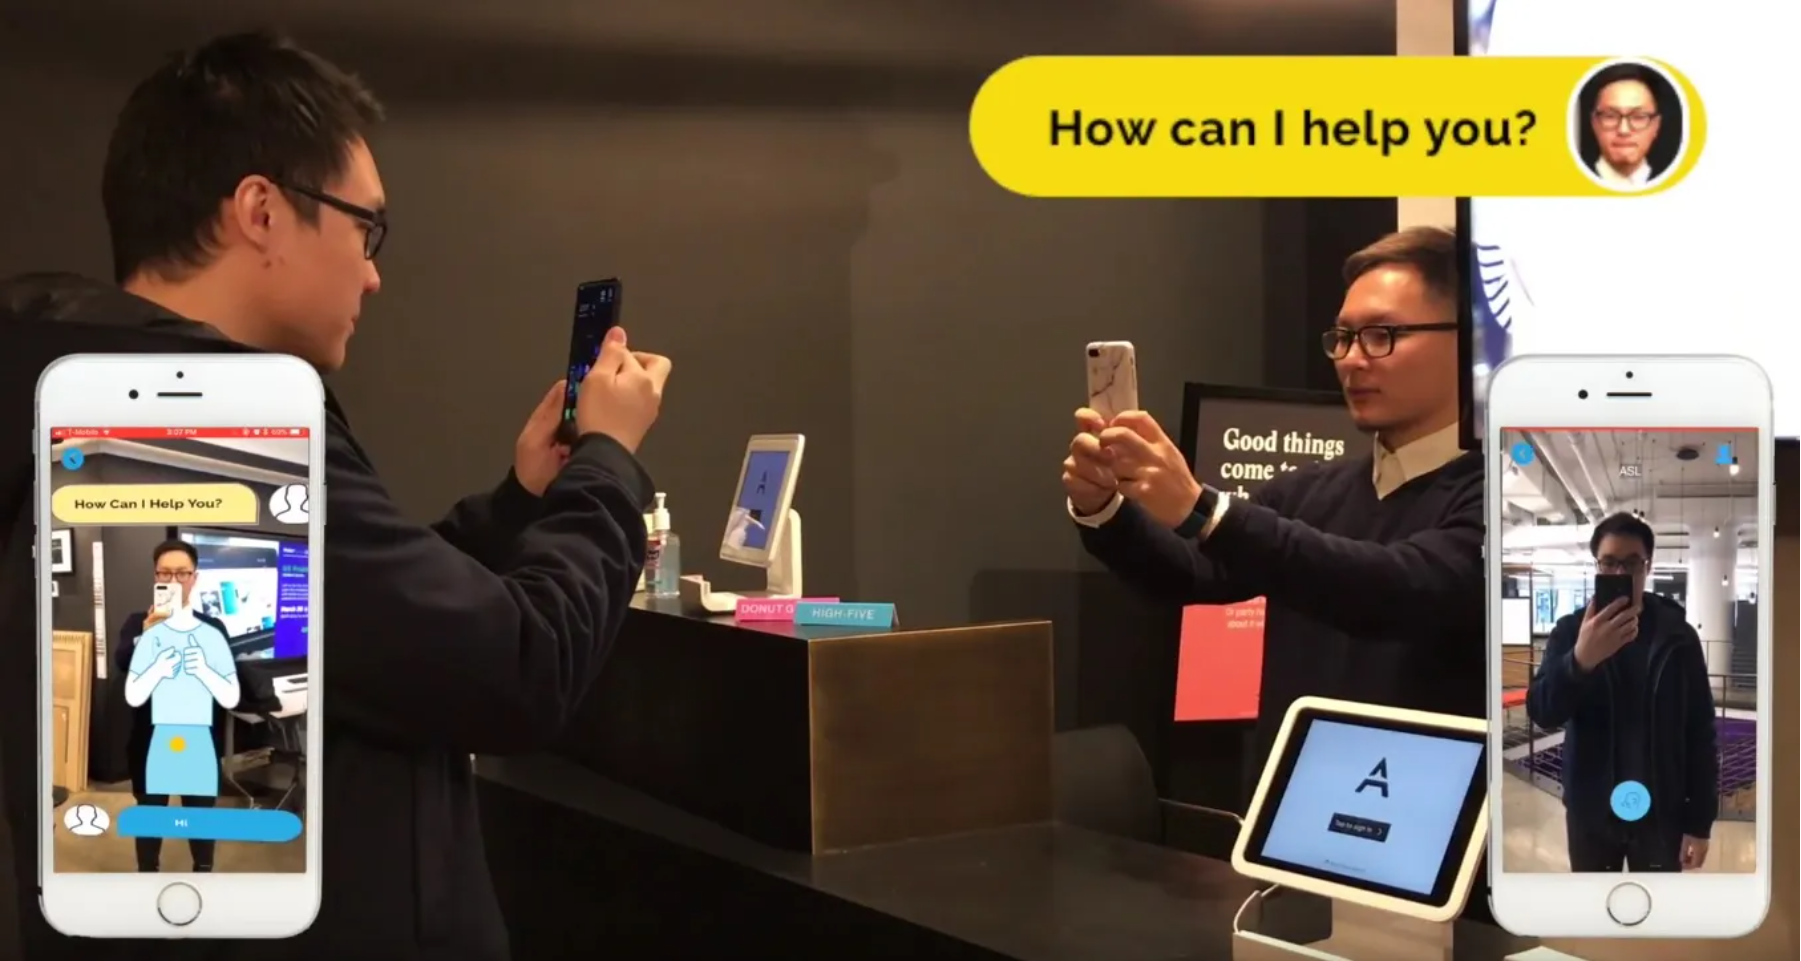
\includegraphics[width=0.45\linewidth]{ASLR.png}}
  \subcaptionbox{AR眼镜上的实时语音翻译应用\label{fig:SLRb}}
    {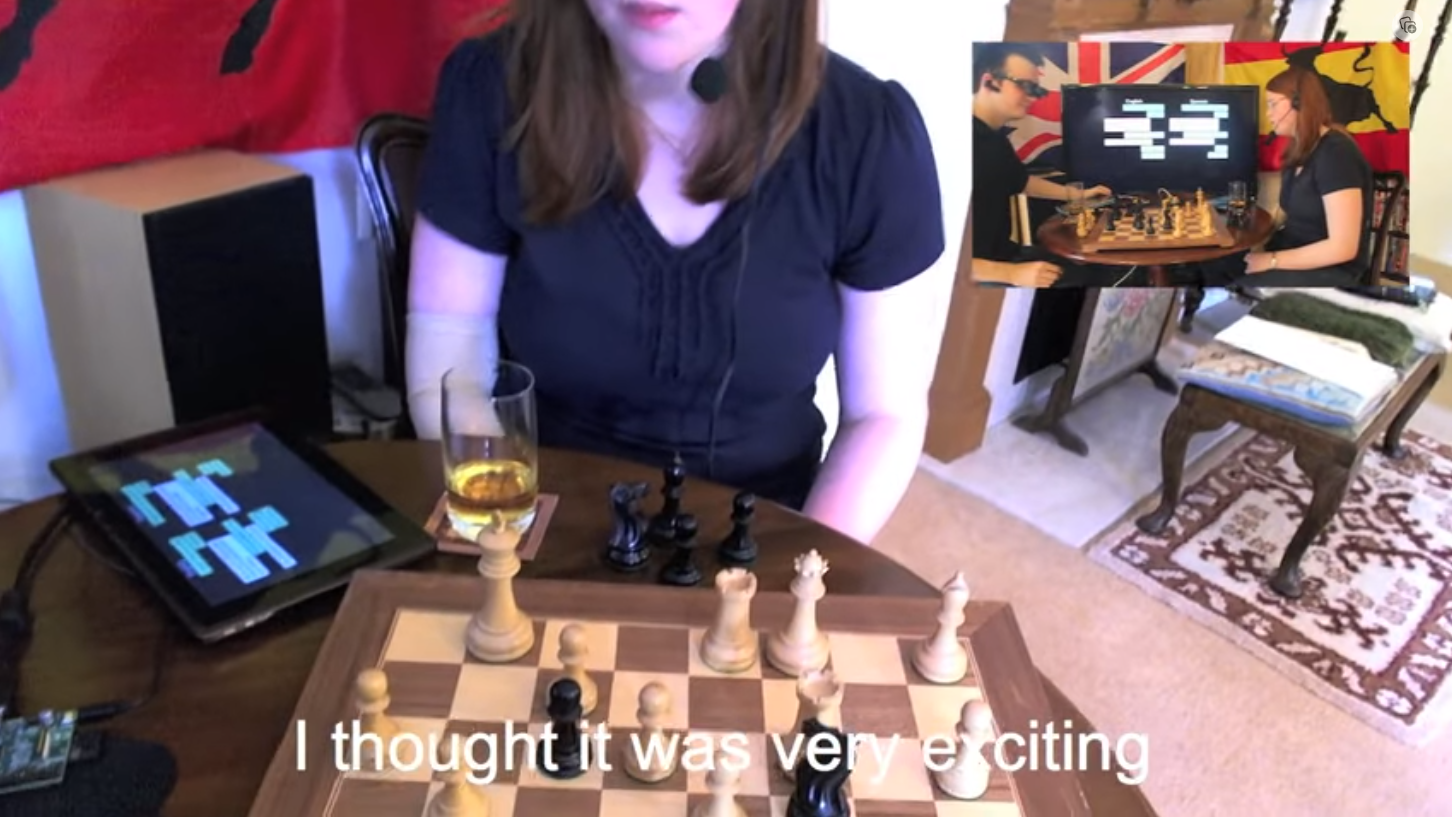
\includegraphics[width=0.45\linewidth]{SLRb2.png}}
  \caption{增强现实环境下的实时翻译应用}
  \label{fig:SLR}
\end{figure}

%【...】
%Birk 等设 计了一个准确率高达 99% 的实时手语识别系统,该系统采用主成分分析法对手势图像 进行特征提取,并基于欧几里德距离完成了贝叶斯分类器的训练[28]。Murugeswari 等基 于单目摄像头采集的图像,采用 SIFT 方法提取手势的关键点,然后使用向量量化将关 键点映射成统一维度的直方图向量,最后利用 SVM 多分类方法完成手势的分类[29]。国 内研究者张良国 等基于 Hausdorff 距离模板匹配的方法,在中国手语手指字母集上基于 单目视觉实现了识别 30 个手指字母的手势识别系统,平均识别率达到了 96.7%[30]。中 国科学与技术大学的黄杰基于三维卷积网络和注意力机制等深度学习方法,针对手语识 别中的孤立手语和连续手语识别进行了详细研究 [31] 。
%[28] BIRK H, MOESLUND T B. Recognizing gestures from the hand alphabet using principal component analysis[J]. 1996. [29] MURUGESWARI M, VELUCHAMY S. Hand gesture recognition system for real-time application[C]// International Conference on Advanced Communication Control & Computing Technologies. 2015. [30] 张良国, 吴江琴, 高文, 等. 基于 Hausdorff 距离的手势识别[J]. 中国图象图形学报, 2002, 7(11): 1144-1150. [31] 黄杰. 基于深度学习的手语识别技术研究[D]. 中国科学技术大学, 2018.

(5)虚拟现实交互。手势能够使用户与虚拟场景的交互更加自然方便,因此被广泛应用于增强现实、虚拟现实等环境中(图\ref{fig:3b})。Taylor等人使用手势识别系统对采集到的手势进行实时匹配以弹奏虚拟钢琴\cite{taylor2016efficient}。
%随着虚拟现实 VR(Virtual Reality)和增强现实 AR(Augmented Reality)技术的发展,用户对于虚拟场景的交互体验要求也越 来越高。手势识别技术的应用能够提升用户体验,使用户与虚拟场景的交互更 加自然方便,如实现三维立体影像操控、虚拟物品的拿取等。
% AR,VR中的手势输入...
% 弹奏虚拟钢琴。该手 势识别系统利用数据集与采集到的手势进行实时匹配[63]。
%[63] TAYLOR J,LUFF B,TOPALIAN A,et al.Efficient and precise interactive hand tracking through joint,continuous optimization of pose and correspondences[J]. ACM Transactions on Graphics,2016,35(4):143.

(6)游戏娱乐。手势识别技术在游戏领域(Kinect、Xbox)得到了广泛应用。例如,通过摄像头传感器捕捉玩家的手部和身体动作,实现与游戏的自然交互,提升游戏体验。
% 腾讯云神图·手势识别。25 种常见的静态手势

(7)临床与健康。手势识别技术可以帮助医生在手术室内实现非接触式操控医疗设备和影像系统\cite{strickland2013using}。同时,该技术也被应用于辅助行动不便人士的康复训练和日常生活,例如通过手势来控制智能轮椅\cite{zeng2012natural}。
% 在临床手术中,为了缩短手术时间或提高结果的精 确性,外科医生可能需要患者整个身体结构的细节或详 细的器官模型,通过使用医学成像系统,如MRI、CT 和 X-ray 系统来实现。这些系统从患者的身体中收集数 据,并将其作为详细的图像显示在高分辨率的电子大 屏。外科医生可以通过使用计算机视觉技术在摄像头 前做手势来观察图像的交互。这些手势能实现一些操 作,如缩放、旋转、图像裁剪和切换到下一张或上一张幻 灯片,而无需使用任何周边设备,如鼠标、键盘或触摸 屏。任何额外的设备都需要消毒,这对于键盘和触摸屏 来说可能很困难。
% 此外,手势可以用于辅助目的,如轮 椅控制[58]。
% [58] ZENG J H,SUN Y R,WANG F. A natural hand gesture system for intelligent human-computer interaction and medical assistance[C]//2012 Third Global Congress on Intelligent Systems,2012:382-385.
% 多伦多Sunnybrook医院[167]伦敦的盖伊和圣托马斯医院[168]都通过精心设计的三维手势此对,实现无菌环境中的非接触式操作。
% (167) Strickland M,Treraine J, Brigley G, et al. Using a depth-sensing infrared camera system to accessand manipulate medical maging from within the sterile operating field(J]. Canadian Journal ofSurgery, 2013,56(3): E1.[168] OHara K, Gonzalez G, Sellen A, et al. Touchless interaction in surgerylJ]. Communications of theACM,2014,57(1): 70-77.

(8)计算机交互。手势交互作为一种创新的人机界面形式,能够取代鼠标键盘等传统设备,为用户提供更加直观的界面操作体验\cite{starner1998real}。
% [65] STARNER T,WEAVER J,PENTLAND A.Real-time American sign language recognition using desk and wearable computer based video[J].IEEE Transactions on Pattern Analysisand Machine Intelligence ,1998,20(12):1371-1375.

% 文献评述
本研究将聚焦动态手势识别与手势生成算法在手语教学中的应用。基于构建的交互式手语学习助手系统,实现手语学习、辅助练习、实时反馈等功能。这不仅能够有效缓解手语教育师资与教学资源短缺的难题,还能提升手语教学中的人机交互体验,具有广泛的社会价值与应用潜力。
% \textcolor{red}{本研究将聚焦动态手势识别算法在机器人控制系统中的应用。结合本研究所提出的先进的多模态动态手势识别算法的优势,我们首次尝试将手势识别应用部署于奥比中光机器人平台环境,构建手势识别控制系统。这不仅能够有效提升人机交互过程中的用户体验,还具有广泛的应用潜力。}

%结合Li\cite{SLR1}和Will\cite{SLR2}等人的设计优势,我们首次尝试将实时手语翻译应用部署于可穿戴增强现实环境。与传统基于手机或电脑的翻译系统相比,基于增强现实眼镜的可穿戴手语翻译系统具备灵活、便携、自然、非侵入式的优势,可以广泛应用于“医疗急救\cite{2022signmedicial}、法律援助\cite{2021signlawyer2}、手语教学\cite{2022signlearning}”等场景。这不仅能够有效提升手语沟通过程中的人机交互体验,还具有广泛的应用潜力。
%国内外研究学者针对XX问题的研究主要集中在A、B、C、D等方面,目前对(选题) 领域的研究相对较少(论文有几个研究内容,这里就有几个研究不足),对(选题) 领域的深入研究能够实现······,丰富......具有重要的理论和应用价值。


\section{研究内容}

本文针对多模态动态手势识别算法与协同手势生成算法进行了研究,并基于此构建了一个交互式手语学习助手。具体研究内容如下:

% \textcolor{red}{添加手势生成的背景}

\paragraph{多模态手势识别算法研究} 针对动态手势识别任务中存在的“信息冗余”与“信息缺失”挑战,本研究提出了一种用于 RGB-D 手势识别的新型可插拔方法,称为多策略解耦和语义集成手势识别网络(Multi-strategy Decoupling with Semantic Integration Network,MDSI)。
% 如图~\ref{fig:MDSI}所示,该算法以动态手势解耦为出发点,旨在提取手势中的多尺度特征,并通过时空注意机制实现高效的时空建模;在此基础上,基于多模态文本编码器集成语义知识,从而显著提升手势识别算法的准确性和泛化性。
首先,为了缓解 IR,我们引入了多策略解耦网络 (MDN)。该网络通过多种策略巧妙地解耦了纠缠的手势特征:a) \emph{姿势-运动解耦} (PMD) 和 b) \emph{空间-时间-通道解耦} (STCD)。
PMD 将手势视频解耦为细粒度 \emph{姿势} 和粗粒度 \emph{运动},由冻结的预训练姿势估计器 \cite{sun2019deep} 支持。
STCD 采用与维度无关的自注意力技术,从而有效地消除了多余的信息并增强了微妙但关键的特征。
其次,为了解决 IA,我们将自然语言建模集成到手势识别中,开发了语义整合网络 (SIN)。SIN 由两个核心组件支撑:\emph{语义过滤器} (SF) 和 \emph{语义标签平滑} (SLS)。SF 采用跨模态混合过滤将语义信息集成到视觉建模中,从而提高了模型在潜在特征空间中辨别细微差别的能力。
SLS 利用标签的语义相似性在训练阶段深化模型的语义理解。
此过程利用强大的预训练 CLIP 文本编码器来提取深度语义特征,编码器在训练期间冻结,不会产生额外的计算成本。
据我们所知,我们是第一个将多模态语义信息引入该领域的,标志着一项有希望的探索。
我们在基准 IsoGD 和 THU-READ 数据集上进行的大量实验结果表明,所提出的方法可以显著提高基于 RGB-D 的手势识别性能。

\paragraph{协同手势生成算法研究} 
% 本文方法
针对手势数据的描述文本缺失和多模态协同控制困难的挑战,我们提出了一种新颖的手势描述与生成(CoordSpeaker)方法,通过手势到描述的转换填补手势语义标注的空白,并通过描述增强的伴随语音手势生成实现对手势生成的精确语义控制。首先,为应对协同多模态控制生成的挑战,我们开发了一个手势潜在扩散模型,该模型包含一个手势变分自编码器(VAE)用于学习统一的动作潜在表示,以及一个具有层次控制去噪器的潜在扩散模型,用于实现精细的多条件控制。其次,为缓解手势数据标注缺失的问题,我们引入了一个手势描述框架,该框架利用动作-语言模型以低成本为手势数据生成描述性文本,并通过多粒度描述控制机制实现精确的语义控制。据我们所知,这项工作是首次探索解决手势语义标注挑战的手势描述方法,从而实现了对手势生成的有效描述和语音控制,为手势-文本双向转换提供了新的视角。大量实验表明,我们的方法能够有效生成描述性手势描述,并实现语义连贯、节奏同步的手势生成。

\paragraph{交互式手语学习助手}
进一步地,本文将深入探讨算法在人机交互中的应用前景。基于所提出的MDSI动态手势识别算法与CoordSpeaker协同手势生成算法构建一个交互式手语辅助学习系统,结合多模态信息融合技术和实时动作捕捉机制,实现精准、高效的手势识别响应,与流畅、自然的手势动作生成。
这不仅有助于改善提升手语教学过程中的人机交互体验,缓解手语教育师资与教学资源短缺的难题\cite{2022signlearning},更可以充分发挥人工智能手势技术在人机交互环境中的潜力,具有广泛的社会意义与应用价值。
%,可部署于可穿戴增强现实环境。相比于传统基于手机或电脑的识别系统,我们的设计具有可穿戴、灵活、非侵入性、自然、移动性强等优势。
% 该系统可广泛应用于“医疗急救\cite{2022signmedicial}、法律援助\cite{2021signlawyer1}、手语教学\cite{2022signlearning}”等领域,提升手势沟通过程中的人机交互体验,具有广泛的应用价值。



\section{章节安排}

本文共分六章,主要内容组织如下:

第一章为绪论,分析了研究背景及意义,介绍了国内外研究现状,并阐述了本文的研究内容和章节安排。

第二章为相关技术,介绍了本文所涉及的计算机视觉基础知识和生成模型基础理论,包括3D卷积神经网络、视觉变换器、变分自编码器和扩散模型等关键技术。

第三章为多模态手势识别算法研究,提出了一种可插拔的多策略解耦和语义集成网络(MDSI),通过解耦视觉特征提取与多模态语义集成,有效解决了RGB-D手势识别中的信息冗余和信息缺失的挑战。

第四章为协同手势生成算法研究,提出了一种基于描述驱动的协同手势生成框架(CoordSpeaker),通过引入可控潜在扩散模型与多粒度手势描述策略,实现了手势生成过程中语义和节奏的协同精确控制。

第五章为交互式手语学习助手设计与实现,基于前述算法,构建了一个可交互的手语辅助学习系统,实现了手语学习、辅助练习、实时反馈等功能。

第六章对本研究的主要工作进行归纳,阐述了研究的创新贡献,并探讨了后续的研究方向。
